
\chapter{相关工作与国内外研究现状}
\label{chapter:relate}

\section{流式学习研究现状}

数据挖掘是一个跨学科的研究领域,用以从大数据中提取模型和模式\cite{hand1999statistics, hand2001principles, nialladamsadvances}
随着机器学习研究的进展,许多数据挖掘分析问题得到了解决。 
针对数据量持续增大的问题,研究者已经提出一些新的存储、机器学习和统计分析技术来处理可扩展性问题。

随着网络和并行计算技术的发展,新的分布式和并行机器学习数据挖掘算法也得到了发展。 
这些算法的目标是从数据集的不同子集中提取知识,并集成这些生成的知识结构,以获得整个数据集的全局模型。
为了缓解通信开销问题,一些客户/服务器,移动代理和混合模型算法也相应地被提出\cite{park2002distributed}。

近年来互联网技术的发展和应用,使得一些数据源中的数据生成速率比以往更快。
这种快速生成的连续数据息流对计算系统中的存储,计算和通信能力提出了挑战。

海量流式数据所带来的问题,通常可以通过两种途径解决,基于数据和基于任务的解决方案。 
在基于数据的解决方案中,算法仅检查整个数据集的一个子集,或将数据垂直或水平变换为近似较小的数据表示。
另一方面,在基于任务的解决方案中,通常采用计算理论的技术来实现时空效率的解决方案。

\subsection{基于数据的方案}
基于数据的方案通常指通过对整个流入的数据集者选取子集或者进行总结的方式来进行分析。
Sampling(采样), shedding和sketching是三种常见的选取子集的方式。摘要和汇总属于进行总结的方式。

\subsubsection{Sampling}
采样(Sampling)是指按照某中概率分布确定某一样本是否被选取的过程。
采样还可以细分为:领域采样,全局采样,水库采样以及不同采样。
在机器学习中如果使用采样策略,则计算误差的边界是采样率的函数,并使用Hoeffding边界来估计样本采样大小\cite{domingos2001general}。

采样算法的应用常见于如下问题:
\begin{itemize}
\item 在Cash Register数据流中查找不同项目的数量。见\cite{gibbons2001distinct}。
\item 在Cash Register数据流中查找分位数。有关最新的结果,请参见\cite{greenwald2001space}。
\item 在Cash Register数据流中查找频繁的项目。见\cite{manku2002approximate}。
\end{itemize}
 
这些问题都有很好的应用(除了上面引用之外还有很多其他的应用)。
此外,在高速流数据上实施采样也是相当实际的。 
(事实上,在一些监控数据流的系统中 - 特别是IP数据包嗅探器 - 
对流进行采样,只是为了将速率降低到合理的水平,但是一般都会按照某种既定的方式进行,否则有价值的信号可能会丢失。)
另外,保留样本有助于估计许多不同的统计信息。

在流式场景下,使用采样的问题是数据的大小无法提前预知。
因此,需要进行特殊的分析以找到误差边界。采样的另一个问题是,在一些问题场景中数据的异常对任务的影响很大,此时采样可能不是一种好的选择。
采样也不能解决数据速率波动的问题。

\subsubsection{Shedding}
Shedding指的是丢弃一些数据流序列的过程,在查询数据流应用中有比较广泛的应用\cite{babcock2003load, tatbul2003load}。
但是存在和Sampling类似的问题,并且难以应用到数据挖掘算法中。
因为,这种方法丢弃的数据会使得破坏数据的结构性,从而使得算法模型无法得到好的模式。

\subsubsection{Sketching}
Sketching主要依赖于降维,是对样本特征子集进行随机选取的过程,也就是数据流的垂直采样。
这种方法通常适用于Turnstile模型,因此非常普遍。

Indyk\cite{indyk2000stable}基于工作\cite{alon1996space}提出使用稳定分布来生成随机变量,具有不同稳定分布的Sketching相当于估计了数据流上的不同$L_p$范数。
比如使用高斯随机变量的Skeching可以很好地估计数据流的$L_2$范数,使用Cauchy分布可以得到$L_1$范数的良好估计。

Sketching还有许多变形,这些变形一般更为简单。 例如,随机子集\cite{gilbert2001surfing},Counting Sketches\cite{charikar2002finding}
以及Bloom filters\cite{broder2004network}。


从稳定的分布中采样产生一个随机变量序列的强大之处在于,这样一来,可以根据需要快速总结得到给定范围的属性。
而事实上这样的构造方法存在,并且可以快速生成样本并使用小空间。比如\cite{feigenbaum2002approximate}论文中提到的方法,\cite{gilbert2001surfing}中的Reed-Muller构造,
\cite{gilbert2002fast}中的$L_1$和$L_2$ Sketches的一般构造,以及\cite{cormode2003estimating}中$p\rightarrow0$的稳定分布的构造方法。

这种方法的主要缺点在于准确率,在一些场景中主成分分析会比这种方法更有效。

\subsection{基于任务的方案}
基于任务的技术是指那些为了解决流式计算挑战而修改或提出的新技术。近似算法,滑动窗口以及算法输出粒度属于这一类。

\subsubsection{近似算法}

近似算法\cite{muthukrishnan2005data}根源在于算法设计。它涉及计算难题的算法设计。 这些算法可以产生具有误差边界的近似解。
这种思路考虑到受到流式数据特性,在流式数据上的挖掘算法本身就是一个很难的问题。
近似算法作为解决流式数据机器学习和挖掘的解决方案,已经吸引了许多研究人员的兴趣\cite{cormode2005s}。
然而,近似算法并不能解决流式数据的速率的问题。

\subsubsection{滑动窗口}
使用滑动窗口技术的思想很自然,因为通常用户更关注最近数据。MAIDS\cite{dong2003online}系统使用了许多对于最近的数据的分析和总结技术。

\subsubsection{算法输出粒度}
算法的输出粒度(AOG)\cite{gaber2005board, gaber2004cost, gaber2004towards}引入了第一个资源感知的数据分析方法,可以根据存储器和时间约束来处理速率波动非常高的流式数据。
AOG在资源受限设备上执行本地数据分析。AOG有三个主要阶段。前两个阶段分别是适应资源和数据流速率,以及执行挖掘。
第三个阶段是在内存不足时合并生成的知识结构。 AOG已被用于聚类,分类和频率计算等任务中\cite{gaber2005board}。

\subsection{相关的技术}
流式数据被定义为具有超大规模,持续实时的数据。因而通常无法被完整地存储。
由于流式数据持续特性,数据的分布会受到概念迁移的影响\cite{minku2011online}。
执行在线数据流机器学习的主要要求是随着数据到达而同时做出更新学习的能力。
常见的机器学习算法如决策树是基于批量训练的,在进行训练之前需要大批量数据。
如果发生概念迁移,则需要重新训练模型\cite{zliobaite2011moa}。

在线学习是一种机器学习方法,在其学习过程中,数据一序列的顺序地输入,每条数据都会即使反馈并更新现有的模型。
与其相对应的批量学习则是每次没遍历完所有的训练集才会更新一次模型。
咋期限学习在机器学习领域中是一种常用的技术。在计算无法覆盖整个数据或者需要动态更新模型的情况下尤其适用。

在上世纪50年代,Rosenblatt\cite{rosenblatt1958perceptron}就已经提出了使用在线学习方法来实现感知器(perceptron)算法,可以解决线性可分问题。

流式学习和在线学习有着许多关联。可以说流式学习是在线学习的特例,数据都是按照一定步骤持续输入的,同时需要在线地更新模型。
除此之外,流式学习一般会受到资源的限制,而在线学习则没有明确的约束。

批量学习算法使用批量的训练数据来训练模型。然后使用训练出来的静态模型预测测试集上的样本。在线学习算法则初始化一个随机模型,
之后从训练群体中拾取一个观测样本,并重新校准每个输入参数的权重。

\begin{figure}[htb]\centering
  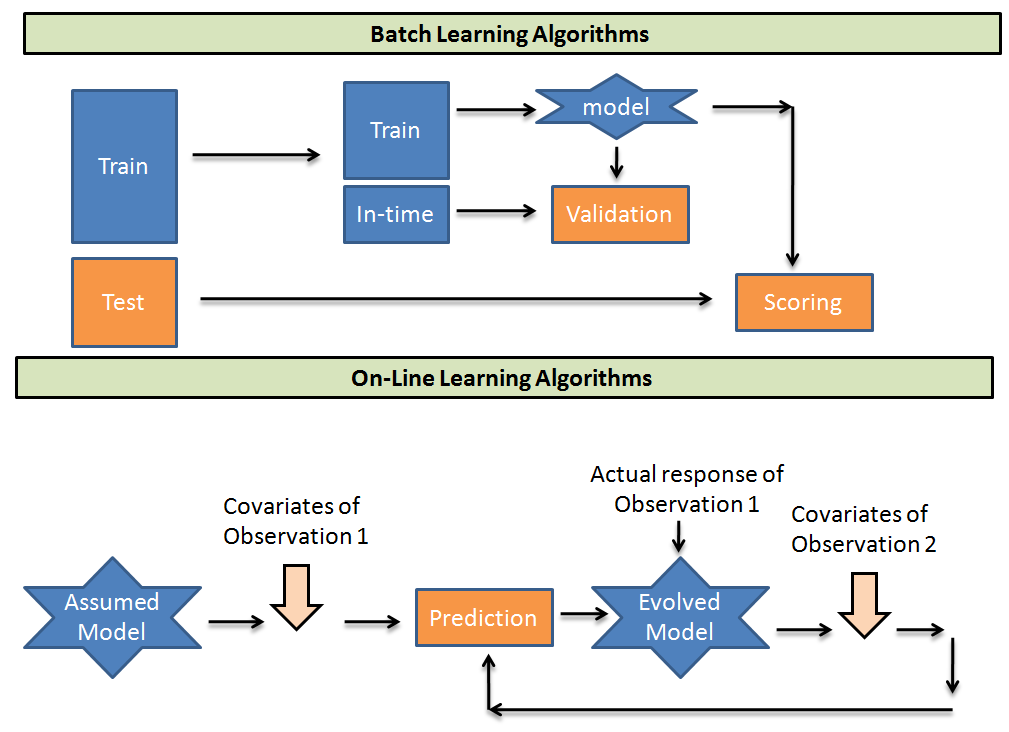
\includegraphics[width=0.7\linewidth]{batch-online}
  \caption{批量学习与在线学习方法对比}
  \label{fig:batch-online}       % Give a unique label
\end{figure}

增量式学习近来受到学术界和行业的日益关注。 从计算情报的角度来看,增量学习至关重要的至少有两个主要原因。
首先,从数据挖掘的角度来看,目前许多数据密集型计算应用需要学习算法能够从大型动态流数据中进行渐进式学习,
并随着时间的推移建立知识库,以使未来的学习和决策受益匪浅 处理。 第二,从机器智能的角度看,生物智能系统能够逐步学习信息。

\section{主题模型研究现状}
主题模型在机器学习和自然语言处理等领域是用来在一系列文档中发现潜在语义的一种统计模型。
其目标是高效第处理大型集合,并找到集合成员的表达,同时保留对基本任务(如分类,异常检测,总结以及相似性和相关性判断)有用的基本统计关系。

信息检索领域的研究人员最早在这类问题\cite{baeza1999modern}取得了重大进展。
IR研究人员为现代互联网搜索引擎成功部署的文本语料库提出的基本方法 - 将语料库中的每个文档表达为实数向量,每个元素都代表某个计量比。 
在流行的tf-idf方案\cite{salton1986introduction}中,研究者选择了基本词汇表,并且计算语料库中的每个文档,每个单词的出现次数。
在适当的归一化之后,将词频乘上逆文档频率(逆文档频率计数测量整个语料库中单词的出现次数)。
最终结果是得到一个词-文档矩阵$X$,其列包含语料库中每个文档的tf-idf向量。因此,tf-idf方案将任意长度的文档减少到固定长度的数字列表。

虽然tf-idf的规约具有一些吸引人的特征,该方法对维度的规约程度较小,并且难以表达文档内外部之间的交互信息。
为了解决这些缺点,IR研究人员还提出了几种其他降维技术,最著名的是潜在语义分析(LSA)\cite{deerwester1990indexing}。
LSA使用矩阵奇异值分解将tf-idf特征空间分解为多个线性子空间,同时保留了矩阵的大部分方差。
这种方法可以在大型集合中实现显著的压缩。 此外,Deerwester等人 认为LSA分解得到的特征是原始tf-idf特征的线性组合,捕捉到了一些基本语言概念,如同义词和多义词。

\begin{figure}[htb]\centering
  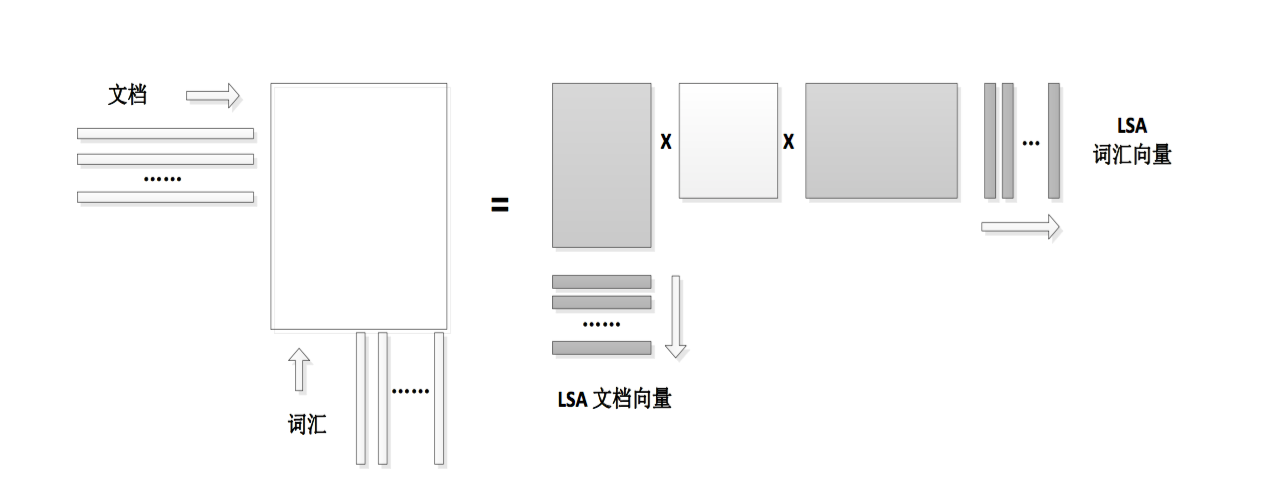
\includegraphics[width=1\linewidth]{LSA}
  \caption{LSA 对词文档矩阵的分解示意}
  \label{fig:LSA}% Give a unique label
\end{figure}

\subsection{主题模型简介}
1999年,Hofmann在论文\cite{hofmann1999probabilistic}中,提出了pLSA模型的重要工作,奠定了主题模型的基础。
PLSA 的出现和上世纪 90 年代兴起的潜在语义分析技术(LSA)有很大的关联,PLSA 可以看作是 LSA 模型在数理统计方面的扩展。
PLSA 简洁的模型让人更加 容易接触,并且使用概率统计知识对模型进行了论证使得模型有了更坚实的理论 基础,
并且 PLSA 模型的算法易于实现,可以适应分布式并行运算,适应了大数 据与分布式计算的时代潮流,最终使得 LSA 得到了强化和推广,大大地推动了 主题模型的研究浪潮。

PLSA方法将文档中的每个单词作为混合模型的样本进行建模,其中混合组件是可以被视为“主题”表示的多元随机变量。
因此,每个单词都是 从单个主题生成,并且可以从不同的主题生成文档中的不同单词。 
每个文档被表示为这些混合组分的混合比例的列表,从而映射到固定的主题集合上的概率分布。这种分布式表达可以用于表达文档特征。

\begin{figure}[htb]\centering
  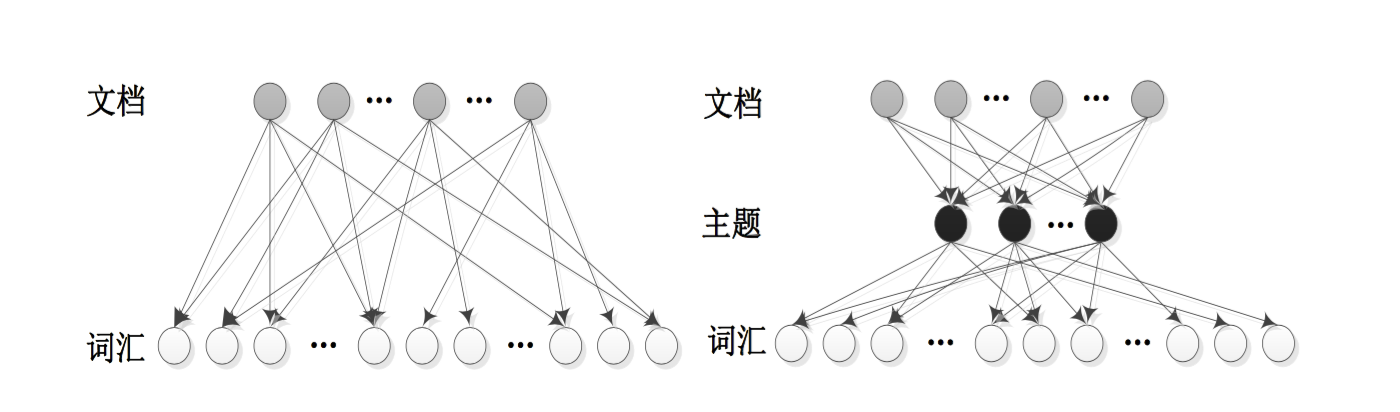
\includegraphics[width=0.9\linewidth]{topic-model}
  \caption{从词文档共现到引入潜在主题的概率模型}
  \label{fig:topic-model}% Give a unique label
\end{figure}

迄今虽然 只有十几年的历史,但是主题模型已经得到了很大的发展,在信息检索、文本分 类和信息抽取等自然语言处理领域得到了很广泛的应用,目前已经延伸至生物信 息学等其他领域。
在PLSA模型中,每个文档被表示成一系列主题概率分布,并且没有针对这些概率的生成模型。
这导致了以下两个主要问题:

(1) 模型的参数会随着训练数据的大小线性增长,不仅参数规模太大,还容易过拟合。

(2) 模型并没有明确给出如何给一个在训练集之外的文档分配概率。

LDA(Latent Dirichlet Allocation Model, LDA)\cite{blei2003latent}是主题模型领域的另外一篇经典之作,最初由David Blei, Andrew Ng, 和 Michael Jordan于2003年提出。
目前在各个领域得到了广泛的应用。不同PLSA的频率学派模型,LDA通过生成式模型克服了上面PLSA模型的主要问题。
该模型假设一篇文档主题分布是由Dirichlet先验分布生成的,同样一个主题下的词汇的分布也是由一个Dirichlet先验分布式生成的。

\subsection{主题模型扩展变形}
在LDA模型提出之后,主题模型再次引起了广泛的关注。研究者又提出了许多LDA模型的变形和改进模型。

Blei等人提出的DTM(Dynamic Topic Model, DTM)\cite{blei2006dynamic}可以捕获在序列组织语料上的主题演变过程。
论文\cite{wang2012continuous}提出了cDTM(Continuous Dynamic Topic Model, cDTM)对DTM进行了改进,使得模型的演变是连续的,而不是对时间进行了离散的分片。
论文\cite{wang2006topics}中也提出了时间上演变的主题模型,该模型显式地将时间建模到模型中去,并且没有做Markov假设。

主题模型通常基于"bag-of-words"假设,在这种假设中词汇之间相互独立,词顺序也相应地被忽略。
这对于那些n-gram模型来说是一个巨大的缺陷。
Wallach的工作\cite{wallach2006topic}提出了一个层次概率生成模型,该模型结合了2-gram的词组和unigram的主题模型,使得模型具有多元词组层次结构。

BTM(Biterm Topic Model, BTM) \cite{yan2013biterm}是主题模型的一种扩展,该模型考虑到了普通的主题模型比较适用于长文档,而对于短文本容易出现文档词共现稀疏的问题。
这种情况在Twitter和微博等场景中尤其常见。因而,模型参考了主题模型的思想在语料集合上构建二元词对集合,这种模型利用直接使用了词共现信息比LDA等模型得到词表达更能够反应词相关性。

在应用方面,主题模型同样有着非常多的变形。其中一些就是情感分析,用于分析文本语义的情感倾向性。
情感主题模型(Topic Setiment Model, TSM)\cite{mei2007topic}以及JSM(Joint Sentiment/Topic Model, JSM)\cite{lin2009joint}都提出了情感和主题混合的模型。
Titov和McDonald\cite{titov2008modeling, titov2008joint}采用了有监督信息并结合情感主题使得模型能够总结情感信息和文本。
除此之外,还有许多主题模型在情感分析领域的应用\cite{lu2011multi, jo2011aspect, li2010sentiment, si2013exploiting}。
在命名实体\cite{han2012entity, newman2006statistical, shu2009latent, kim2012etm}和学术作者识别\cite{rosen2004author}等工作中,主题模型一样得到了很好的应用。带有
带网络结构的主题模型(Topic Model with Network Sturcture, TMN)\cite{mei2008topic}是一种带有网络结构信息的文本主题模型。这种模型从用户角度考虑到互联网文本信息通常带有网络并对此建模。

不仅在文本类型的数据中,主题模型在其他类型的数据上也得到了应用,比如Fei-Fei Li等人将主题模型应用于图像分析\cite{fei2005bayesian, sivic2005discovering}, 
Pritchard\cite{pritchard2000inference}和Erosheva\cite{erosheva2002grade}将主题模型应用于人口调查。
据此,许多研究者都提出了类似的工作,加入上下文信息\cite{mei2006mixture}、时间\cite{wang2006topics}、地理位置和作者信息等等。

\subsection{大规模可扩展的算法应用}
上面的绝大多数数主题模型的工作都是在LDA模型的基础之上提出的。

最初LDA\cite{blei2003latent}提出的模型求解方法是变分推理(Variational Bayesian Inference, VB)\cite{jordan1999an},
这种方法引入了变分参数并利用Jensen不等式使得LDA模型变得更容易求解。
Griffiths\cite{griffiths2004finding}的CGBS(Collapsed Gibbs Sampling, CGBS)方法采用Gibbs采样的方法来求解模型参数。
Blei等人最初提出的VB方法相比,Griffiths的方法中采样空间是一个折叠的空间(通过积分消除了模型参数)使得模型的求解更适合于大数据的应用。
Teh\cite{teh2006a}等人参考了CGBS的工作提出了CVB方法(Collapsed Variational Bayesian Inference, CVB),这种方法不仅使得模型求解更加简便,
同时得到了比Blei等人的VB方法更好的误差下界,因而CVB方法拥有比VB方法更少的假设和约束。

FCGBS(Fast Collapsed Gibbs Sampling, FCGBS)\cite{porteous2008fast}针对CGBS优化方法采样效率较低(每次采样均的时间复杂度为O(K))的问题,提出了更快的算法。
类似的对采样进行加速的方法还有SparseLDA\cite{yao2009efficient}和AliasLDA\cite{li2014reducing}。

互联网海量规模的语料相对于精心设计的,清洗过的小数据来说要复杂得多。
在很多场景中,我们需要维持很大的词汇表和主题个数。因为小模型容易造成一些长尾低频词语义的丢失。
为了适应海量规模的数据和超大规模的参数,通常可以使用分布式并行策略来实现LDA模型(将数据分割存储在不同的机器结点上然后执行并行算法)。
这种方案可以在数千台机器数十亿篇文档上训练拥有上亿参数规模的模型\cite{Liu:2011:PPL:1961189.1961198, Peacock, ahmed2012scalable, li2014scaling, yuan2015lightlda}。 

YahooLDA\cite{ahmed2012scalable}和其它一些参数服务器分布式并行LDA实现\cite{li2014scaling},将词-主题共现计数作为全局共享的参数存储在参数服务器上。
而实际上这些参数会被存储在不同的机器上,从而使得参数规模可以达到更大。
另外,在分布式实现中数据被分成若干个子集存在不同机器结点上,每个子集上的词汇子集相比于全局的词汇表要小很多,因而在请求参数时模型只需要数据所需的部分参数即可。

LightLDA\cite{yuan2015lightlda}采用稀疏和稠密混合的参数服务器设计提高了内存和CPU效率,并且使用Word Proposal和Doc Proposal交替的方式使得采用时间效率达到了O(1)。

\section{本章小结}

本章主要介绍了流式学习和主题模型的相关工作与研究现状。

近年来,一些数据源的数据生成速率比以往更加快速,海量流式数据的机器学习和数据挖掘成为了许多研究者的研究热点。
针对流式数据的机器学习和数据挖掘主要分为基于数据的方案和基于任务的方案。
其中基于数据的方案主要包括采样,Shedding和Sketching等技术;基于任务的方案主要包括近似算法,滑动窗口和算法输出粒度等。
除此之外还介绍了在线学习和流式学习的关系和应用。

主题模型在信息检索和其它许多领域有着广泛的应用。针对不同的任务应用主题模型有许多响应的改进和扩展。
目前最为流行和应用最广的主题模型当属LDA模型。
在互联网海量数据的背景下,简单的LDA求解方式如CVB何CGBS方法效率和扩展性都太低。
研究者相应地提出了高效率,扩展性强的算法,如YahooLDA, PLDA+, Peacock以及LightLDA。这些工作实现了超大规模的LDA模型训练。
